\subsection{Parametervariasjon}
\subsubsection{Endring i spennkraft}

\begin{figure}[H]
	\centering
	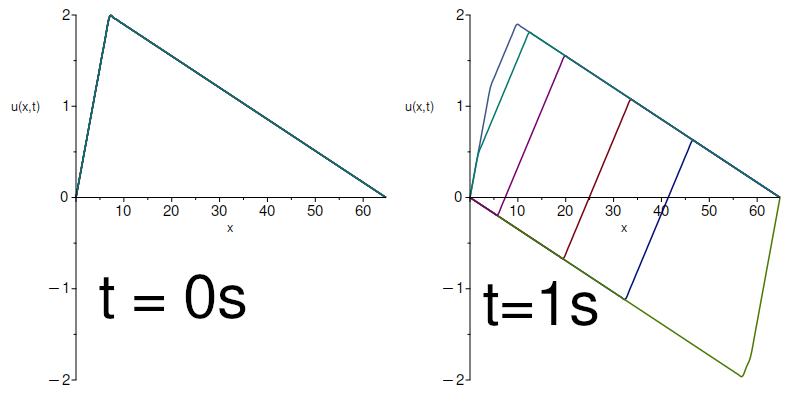
\includegraphics[width=0.8\textwidth]{figurer/MapleSimulering0sog1s.png}
	\caption{Gitarstrenger ved t=0s og t=1s}
	\label{fig:mapleSim0sog1s}
\end{figure}

Initialbetingelsene for figur (\ref{fig:mapleSim0sog1s}) er de samme som gitt i metodekapittelet. Alle 
strengene starter med samme initialfunksjon $f(x)$, det eneste som er ulikt mellom grafene er strengspenning
og massetetthet. Ettersom at det ikke var mulig å legge til navn for de ulike grafene, er det vanskelig å
skille mellom de ulike strengtykkelsene og strengspenningene. 

Her er en liste over de ulike strengtykkelsene, massetethetene og $c$-verdiene:

\begin{center}
	\begin{tabular}{|c|c|c|c|}
		 Streng	&	strengtykkelse	&	massetetthet, $\rho$	& $c$-verdienre \\  
	\end{tabular}
\end{center}

\subsubsection{Endring i massetetthet}
\dots

\subsection{Numeriske resultater}
\subsubsection{Resultatgjennomgang}
For å se animasjonsresultatene av den numeriske løsningen kan du besøke denne kilden: \parencite{simuleringVideo}.

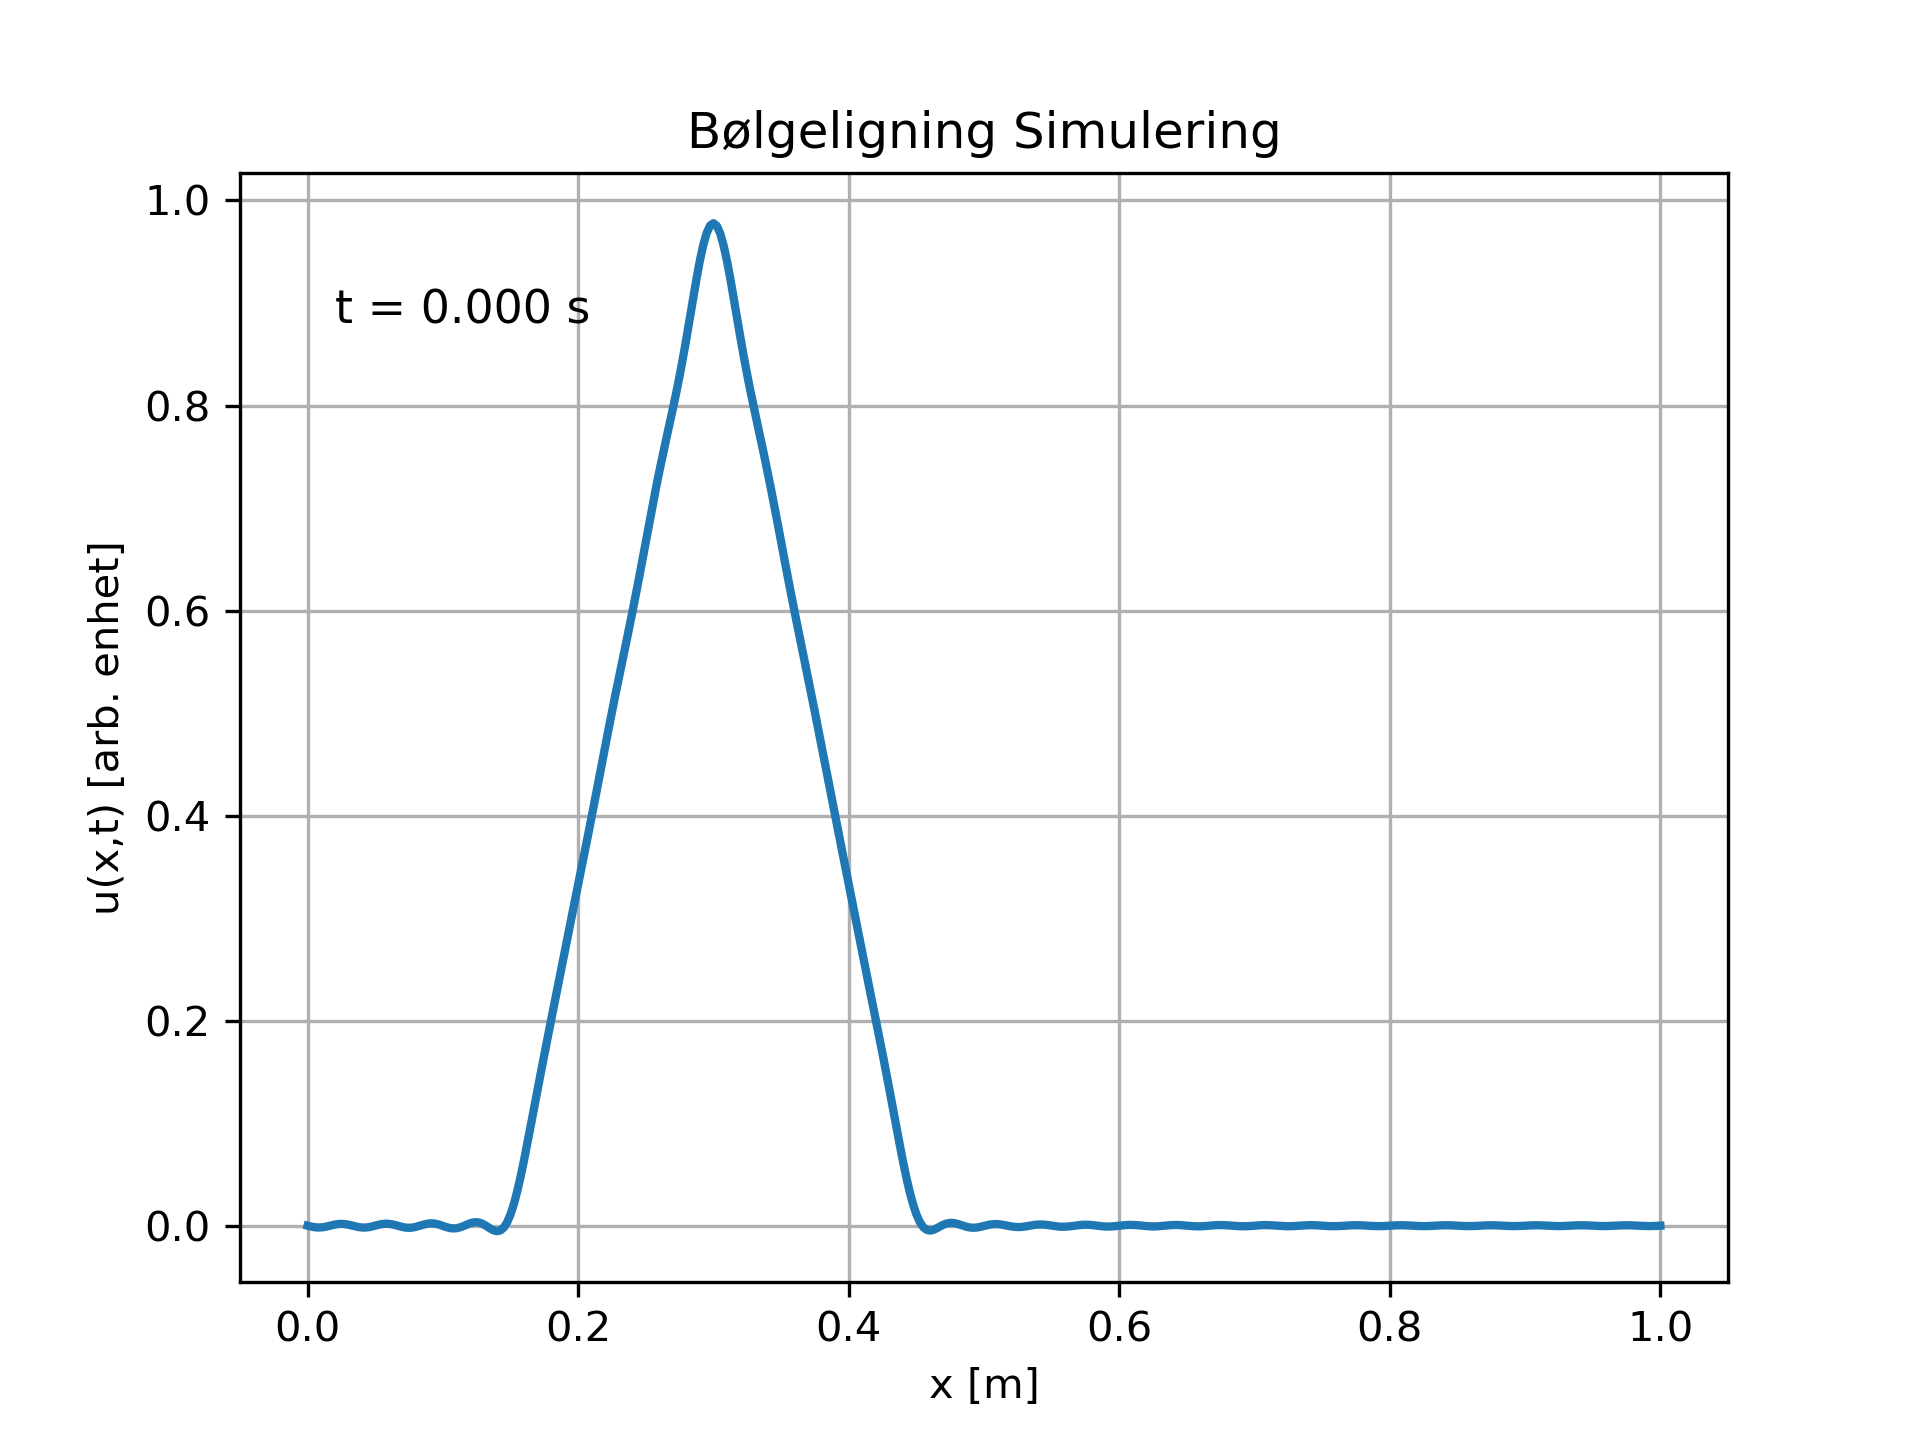
\includegraphics[width=\textwidth]{figurer/bolgeligning_t0.png}

Her ser vi animasjonen for den numeriske løsningen ved t=0 som er lik initialformen som blir satt. Dette er fordi initialfarten er satt til $0$.
Slik som nevnt tidligere vil dette da være et trekantformet "plukk" som  har bredde $0.3m$, som starter i $x=0.15$ og ender i $x=0.45$. Vi 
vet også fra koden at vi har satt $N=60$, dette er en høy nok verdi til at løsningen nærmer seg konvergering for Fourierserien og nær den trekantformen som vi har satt i 
initialbetingelsene. Hvis $N$ hadde vært lavere, eksempelvis hvis $N=5$, så ville bølgen sett slik ut:

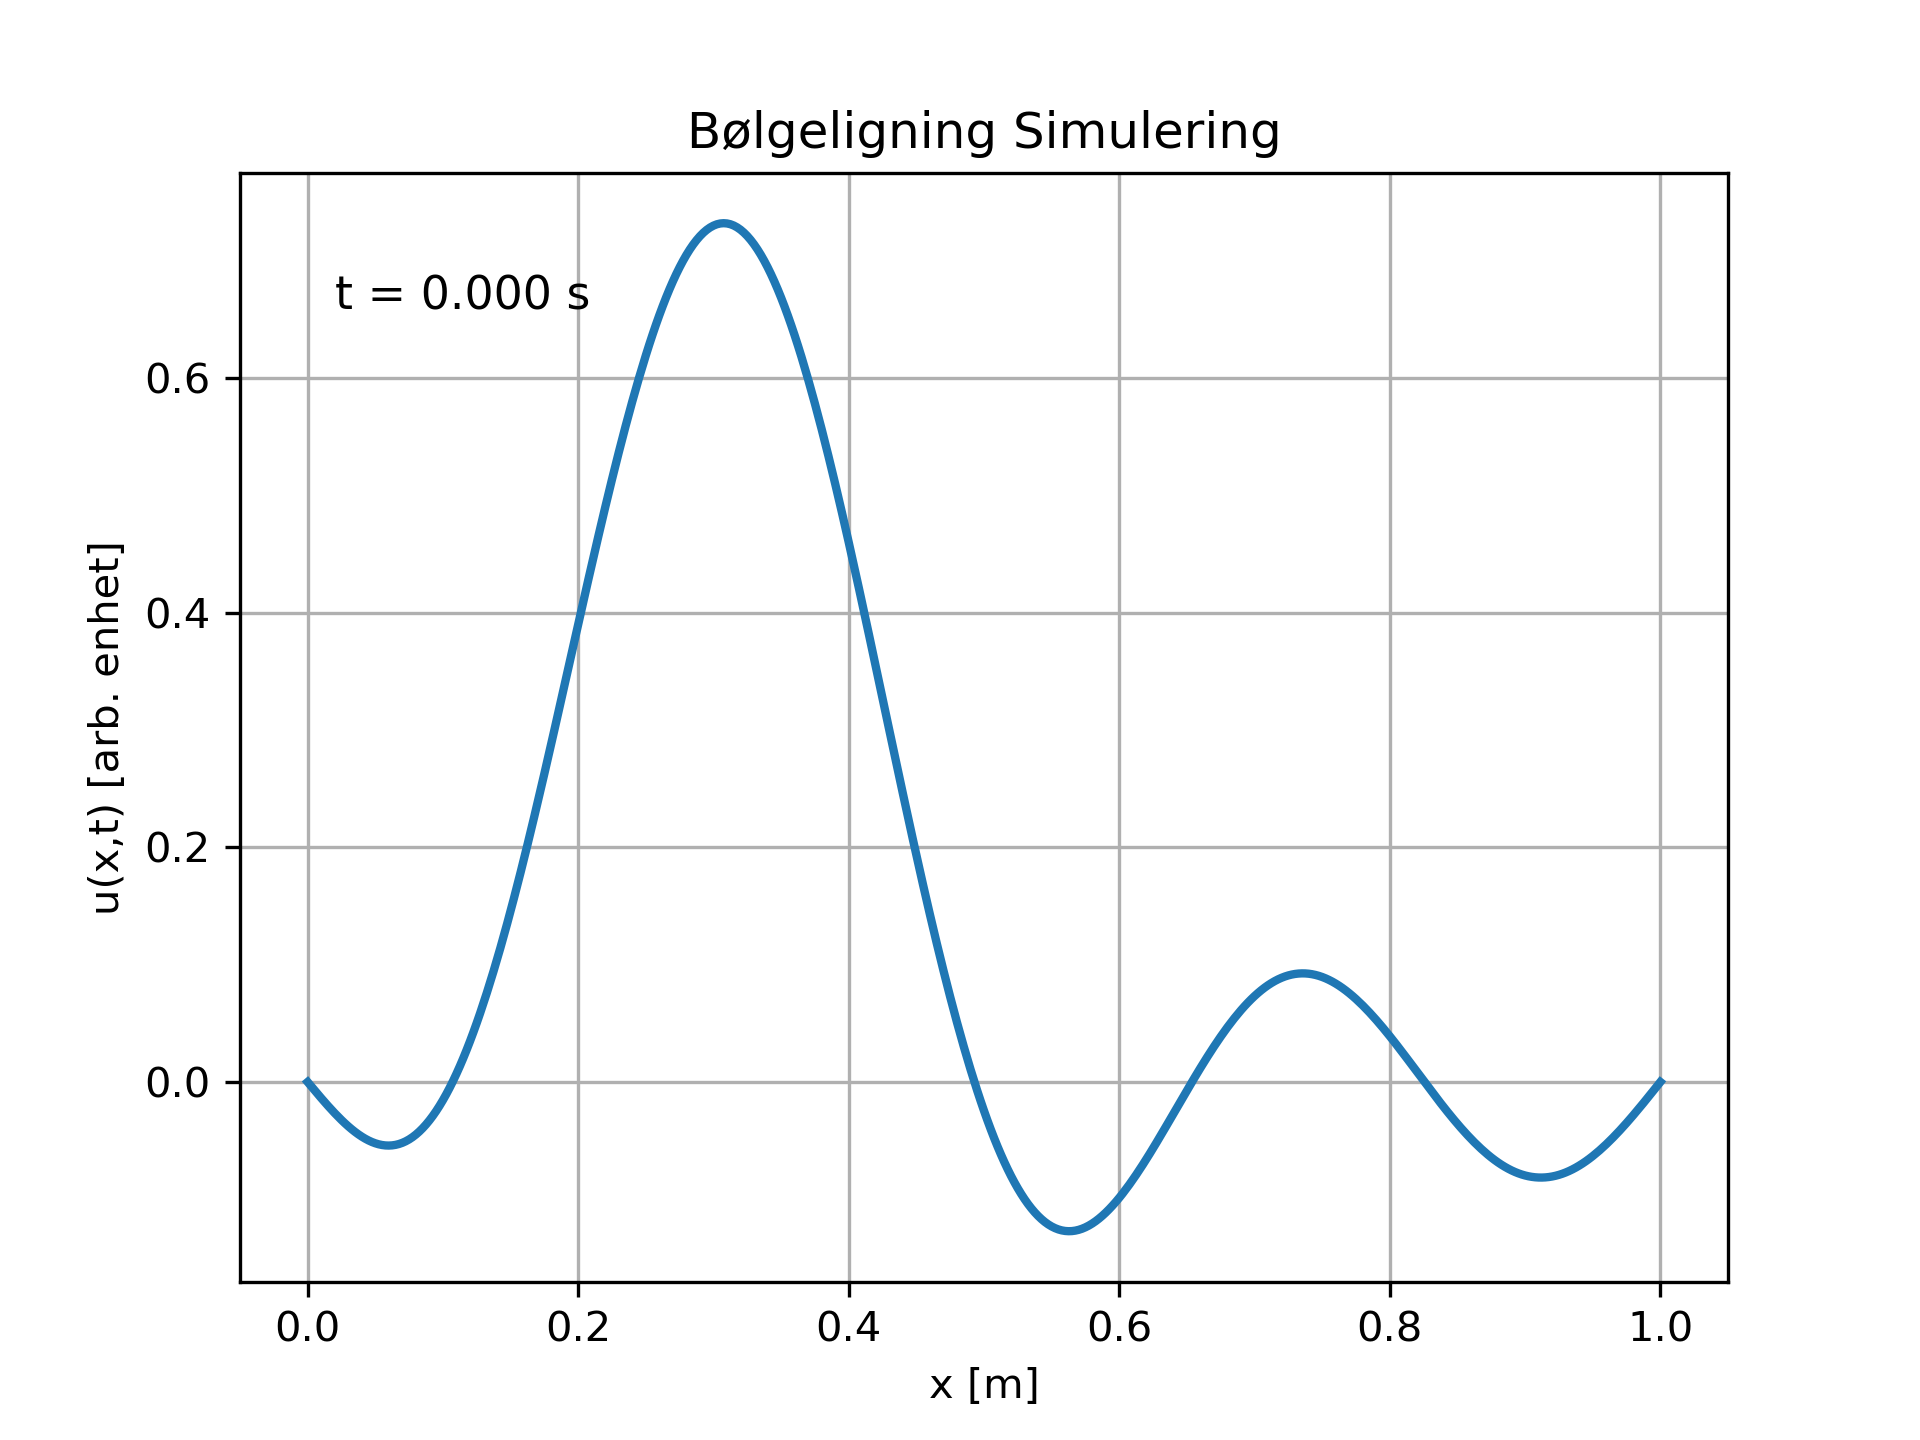
\includegraphics[width=\textwidth]{figurer/bolgeligning_t0_n5.png}

Ved lavere verdier av $N$ (som vist i figuren over) klarer ikke Fourierserien å gjengi knekkpunktet i plukkformen nøyaktig. Dette fører til 
små oversving og bølger rundt toppunktet, kjent som Gibbs-fenomenet. For å unngå dette er $N=60$ valgt, som gir en tilstrekkelig god tilnærming.
Gibbs-fenomenet kommer til syne gjennom synlig oversving i plukkpunktet, og andre ikke-deriverbare punkter. Dette vil være en gradvis bedre numerisk
tilnærming for økende $N$-verdi, hvor $N=60$ er en god balanse mellom nøyaktighet og beregningstid.

Maksamplituden i den numeriske løsningen er noe lavere enn den ideelle verdien på $1.0$ m. Dette kommer av at trekantformen har et knekkpunkt i toppen, 
der funksjonen ikke er deriverbar. Fourierserien består av glatte sinusfunksjoner, og vil derfor jevne ut toppen noe. Resultatet blir en litt lavere og avrundet maksverdi. 
Den ideelle funksjonen ser slik ut:

\begin{equation*}
    u(x,0) =
        \begin{cases}
        \dfrac{x}{pL}, & 0 \le x < pL, \\[6pt]
        \dfrac{L - x}{(1 - p)L}, & pL \le x \le L.
        \end{cases}
\end{equation*}

hvor $p=0.3$. Funksjonen er da kontinuerlig men ikke deriverbar i toppunktet. 

Et viktig punkt å kontrollere i simuleringen er at randbetingelsene overholdes. 
Vi ser fra både figuren og animasjonen at utslaget ved strengens endepunkter forblir null gjennom hele simuleringen, altså $u(0,t)=u(L,t)=0$. 
Dette bekrefter at den numeriske metoden håndterer de faste endene korrekt, slik at ingen uønsket bevegelse oppstår ved grensepunktene. 
At randbetingelsene oppfylles er avgjørende for at refleksjonene ved endene skal skje riktig, og for at stående bølger senere kan dannes på en fysisk konsistent måte.

\subsubsection{Stående bølger og tidsutvikling}
Når stregnen plukkes, og slippes ved $t=0$ begynner den å svinge følge av spennkraften på strengen. Siden \verb|initial_velocity| er satt til en nullverdi, vil bevegelsen starte 
symmetrisk, hvor 2 bølger vil forplante seg i hver retning på strengen med retning bort fra plukkpunktet. Dette ser vi i animasjonen, hvor det er to identiske bølger med halv 
amplitude fra den plukkhøyden. Når disse bølgene treffer endepunktene som er lokalisert ved $u(0,t)=u(L,t)=0$, vil de reflekteres med en hastighet som har motsatt retning, og 
motsatt fortegn på amplituden. De reflekterte bølgene vil overlappe de som beveger seg i motsatt retning, og interferensen mellom disse danner et mønster av stående bølger.
Etter flere refleksjoner og interferens vil strengen stabilisere seg i et mønster av stående bølger. Disse bølgene har noder ved endepunktene, hvor utslaget alltid er null, og
bukker mellom nodene hvor utslaget når maksimale verdier. Mønsteret av stående bølger avhenger av strenglengden, spennkraften, og massetettheten.

Etter omtrent én sekund i simuleringen sees et tydelig invertert plukk sammenlignet med $t=0$, og ved $t=2$\,s er formen tilnærmet identisk med startformen. 
Dette stemmer med den fundamentale svingeperioden for en streng med lengde $L=1.0$\,m og bølgefart $c=1.0$\,m/s, som er gitt ved

\begin{equation*}
T_1 = \frac{2L}{c} = 2.0\,\text{s}.
\end{equation*}

Strengen returnerer altså til sin opprinnelige form etter ett grunnsving, slik den ideelle bølgeligningen forutsier. 
Høyere moduser oscillerer med perioder $T_n = T_1/n$, og bidrar til den komplekse, men periodiske formen som kan observeres underveis.


\subsubsection{Sammenligning av analytisk og numerisk løsning}
\dots

